
\documentclass{article}
\usepackage{tikz}
\usepackage{tkz-euclide} % loads  TikZ and tkz-base
%\usetkzobj{all}
\usetikzlibrary{calc,math}

\begin{document}
\begin{figure}[!ht]
	\begin{center}
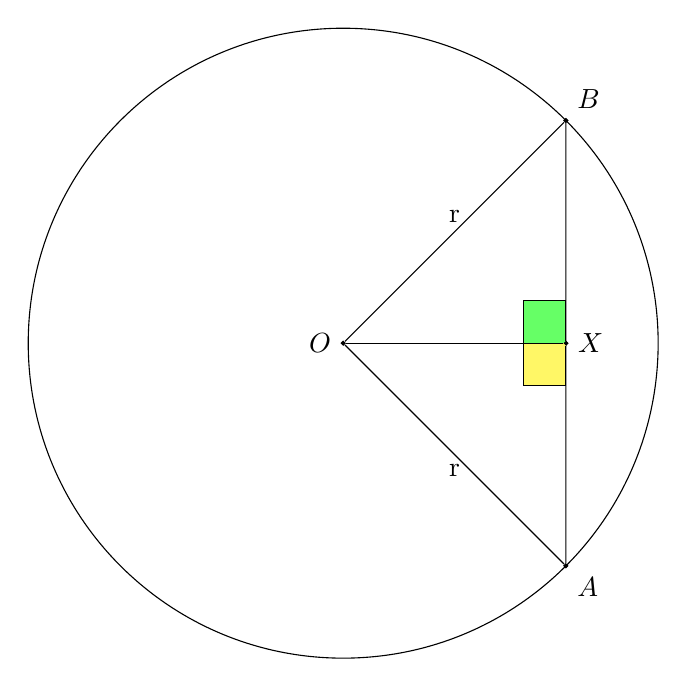
\begin{tikzpicture}
[scale=2,>=stealth,point/.style={draw,circle,fill = black,inner sep=0.5pt},]

%Triangle sides
\def\a{5}
\def\b{6}
\def\r{2}
%Coordinates of A
\def\p{1.414}
\def\q{-1.414}
\draw (0,0) circle (2cm);
%Labeling points
\node (A) at (\p,\q)[point,label=below right:$A$] {};
\node (B) at (\p, \p)[point,label=above right:$B$] {};
\node (X) at (\p, 0)[point,label=right:$X$] {};
\node (O) at (0,0)[point,label=left:$O$]{};
%Foot of median

%\node (D) at ($(A)!0.5!(O)$)[point,label=below:$D$] {};
%\node (E) at ($(A)!0.5!(B)$)[point,label=left:$E$] {};
%\node (F) at ($(C)!0.5!(A)$)[point,label=right:$F$] {};

%Drawing triangle ABC
\draw (A) --  (B) -- node[above] {$\textrm{r}$} (O) -- node[below] {$\textrm{r}$} (A);
\draw (X)-- (O);
%Drawing medians BE and CF
%\draw (D) -- (E);
%\draw (D) -- (F);
%\draw (O) -- (B);
%\draw (O) -- (C);
%Drawing EF
%\draw (E) -- (F);

%Labeling sides
%\node [right] at ($(A)!0.5!(E)$) {$\frac{b}{2}$};
%\node [right] at ($(C)!0.5!(E)$) {$\frac{b}{2}$};
%\node [left] at ($(B)!0.5!(F)$) {$\frac{c}{2}$};
%\node [left] at ($(A)!0.5!(F)$) {$\frac{c}{2}$};

%Angles
\tkzMarkRightAngle[fill=green!60,size=.27](O,X,B)
\tkzMarkRightAngle[fill=yellow!60,size=.27](O,X,A)
%
%\tkzMarkAngle[fill=red!60,size=.7](A,F,D)
%\tkzMarkAngle[fill=red!60,size=.7](A,C,O)
%%
%\tkzMarkAngle[fill=yellow!60,size=.2](A,D,E)
%\tkzMarkAngle[fill=yellow!60,size=.2](A,O,B)
%%
%\tkzMarkAngle[fill=orange!60,size=.2](F,D,A)
%\tkzMarkAngle[fill=orange!60,size=.2](C,O,A)
%
%\tkzMarkAngle[fill=blue!60,size=.3](E,A,F)
\end{tikzpicture}
	\end{center}
\caption{Perpendicular from the center of a circle to a chord bisects the chord}
\label{fig:step1}	
\end{figure}
\end{document}
